\title{%
  SPORES: Transferring files as spores through the wind instead of up in the Cloud
}
\author{Daniel Bosk\thanks{%
    Joint work with Sonja Buchegger (KTH), Adrien Luxey, David Bromberg, 
    François Taîani (INRIA/IRISA Rennes, France)
  }}
\institute{%
  KTH EECS\\
  \email{dbosk@kth.se}
}

\mode<article>{\maketitle}
\mode<presentation>{%
  \begin{frame}
    \maketitle
  \end{frame}
}

\mode*


\section{Introduction}

\subsection{What's the problem?}

\begin{frame}
  \begin{block}{The problem}
    \begin{itemize}
      \item Users have multiple devices: laptop, smartphone, \dots
      \item Files are spread among devices: documents on laptop, photos on phone, 
        \dots

        \pause

      \item Users want to share files.
    \end{itemize}
  \end{block}
\end{frame}

\subsection{Why is it a problem?}
% Why is it a problem? Research gap left by other approaches?
% Why is it important, why care?

\begin{frame}
  \begin{example}[Current practice]
    \begin{itemize}
      \item Alice wants to share a file with Bob.
      \item Alice copies it to Someone Else's computer (a.k.a.\ the Cloud).
      \item She sends a URL to Bob (email, instant message, \dots)
      \item Bob fetches the file from Someone Else's computer.
    \end{itemize}
  \end{example}
\end{frame}

\begin{frame}
  \begin{remark}
    \begin{itemize}
      \item Alice and Bob have privacy against each other.
      \item Someone Else can see everything.
    \end{itemize}
  \end{remark}

  \pause

  \begin{question}
    \begin{itemize}
      \item Can we remove Someone Else's central position?
      \item And still have privacy?
    \end{itemize}
  \end{question}
\end{frame}


\section{The solution}

\subsection{What's the approach?}
% What's the approach? How to solve the problem?

\begin{frame}
  \begin{block}{Goals}
  \begin{itemize}
    \item We want end-to-end encryption for data.
    \item Alice and Bob should only learn that the other has at least one 
      device online.
    \item Someone Else should not learn that Alice and Bob exchange files.
    \end{itemize}
  \end{block}

  \pause

  \begin{idea}
    \begin{itemize}
      \item We leverage that each user have multiple devices.
      \item Although these devices have varying availability.
    \end{itemize}
  \end{idea}
\end{frame}

\begin{frame}
  \begin{block}{Idea}
    \begin{itemize}
      \item We use onion routing with a rendezvous point for privacy.
    \end{itemize}
  \end{block}

  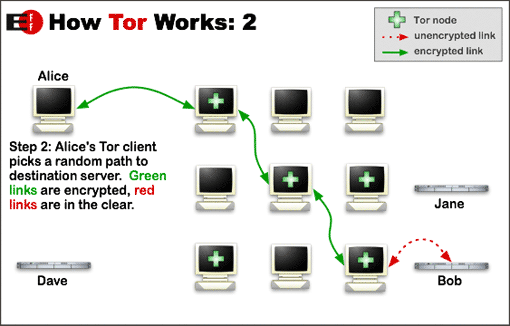
\includegraphics[width=0.48\textwidth]{fig/tor.png}
  \hfill
  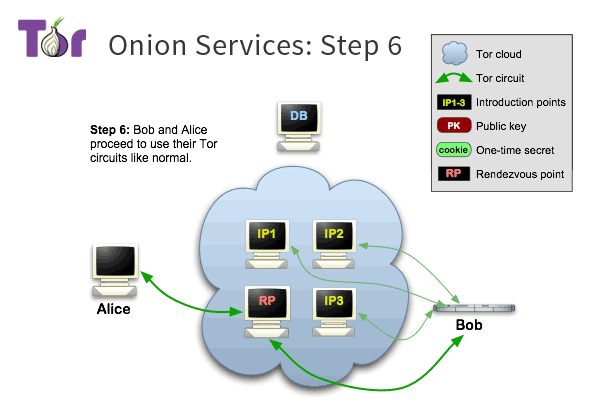
\includegraphics[width=0.48\textwidth]{fig/tor-hs.png}

  \pause

  \begin{remark}
    \begin{itemize}
      \item Our devices are not as reliable as Tor nodes.
    \end{itemize}
  \end{remark}
\end{frame}

\begin{frame}
  \begin{center}
    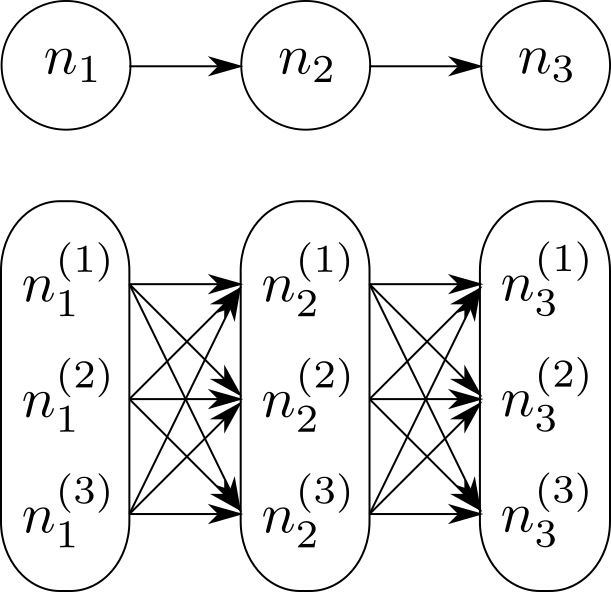
\includegraphics[height=0.5\textheight]{fig/principle-SPOR.pdf}
  \end{center}

  \pause

  \begin{block}{Approach}
    \begin{itemize}
      \item We adapt the Sphinx mix-header format.
      \item Still universally composable.
    \end{itemize}
  \end{block}
\end{frame}

\begin{frame}
  \begin{example}[Scenario]
    \begin{itemize}
      \item Alice wants to send a file to Bob.
      \item \emph{Bob} encodes a SPOR route as a URL and sends to Alice.
      \item Alice \enquote{wraps} a route around Bob's.
      \item She sends the file over the route.
    \end{itemize}
  \end{example}

  \pause

  \begin{remark}
    \begin{itemize}
      \item Bob's set of devices (a squad) must coordinate to reassemble the 
        file.
      \item Alice's squad can coordinate too to send the file.
    \end{itemize}
  \end{remark}
\end{frame}

\subsection{What are the findings?}
% What's the findings? How was it evaluated, what are the results, limitations, 
% what remains to be done?

\begin{frame}
  \begin{block}{Interesting properties}
    \begin{itemize}
      \item Source-bounded random walk
      \item Sender and recipient are sets --- avoids random-walk problems.
      \item Can optimize redundancy for various attributes: availability, 
        bandwidth, \dots
    \end{itemize}
  \end{block}
\end{frame}


\section{Summary}

\begin{frame}
  \begin{block}{Take away}
    \begin{itemize}
      \item Sphinx Extended for Sets (Sphixes)
      \item Onion routing over unreliable nodes.
      \item Alice and Bob can transfer files without Someone Else learning about 
        it.
      \item They reveal minimal information to each other.
    \end{itemize}
  \end{block}
\end{frame}


%%% REFERENCES %%%

\begin{frame}[allowframebreaks]
  \printbibliography
\end{frame}
